\lstset{
	language = Matlab,
	frame = single,
	showstringspaces=false,
	%basicstyle=\ttfamily,
	basewidth={0.55em,0.55em},
	literate={а}{{\selectfont\char224}}1
	{б}{{\selectfont\char225}}1
	{в}{{\selectfont\char226}}1
	{г}{{\selectfont\char227}}1
	{д}{{\selectfont\char228}}1
	{е}{{\selectfont\char229}}1
	{ё}{{\"e}}1
	{ж}{{\selectfont\char230}}1
	{з}{{\selectfont\char231}}1
	{и}{{\selectfont\char232}}1
	{й}{{\selectfont\char233}}1
	{к}{{\selectfont\char234}}1
	{л}{{\selectfont\char235}}1
	{м}{{\selectfont\char236}}1
	{н}{{\selectfont\char237}}1
	{о}{{\selectfont\char238}}1
	{п}{{\selectfont\char239}}1
	{р}{{\selectfont\char240}}1
	{с}{{\selectfont\char241}}1
	{т}{{\selectfont\char242}}1
	{у}{{\selectfont\char243}}1
	{ф}{{\selectfont\char244}}1
	{х}{{\selectfont\char245}}1
	{ц}{{\selectfont\char246}}1
	{ч}{{\selectfont\char247}}1
	{ш}{{\selectfont\char248}}1
	{щ}{{\selectfont\char249}}1
	{ъ}{{\selectfont\char250}}1
	{ы}{{\selectfont\char251}}1
	{ь}{{\selectfont\char252}}1
	{э}{{\selectfont\char253}}1
	{ю}{{\selectfont\char254}}1
	{я}{{\selectfont\char255}}1
	{А}{{\selectfont\char192}}1
	{Б}{{\selectfont\char193}}1
	{В}{{\selectfont\char194}}1
	{Г}{{\selectfont\char195}}1
	{Д}{{\selectfont\char196}}1
	{Е}{{\selectfont\char197}}1
	{Ё}{{\"E}}1
	{Ж}{{\selectfont\char198}}1
	{З}{{\selectfont\char199}}1
	{И}{{\selectfont\char200}}1
	{Й}{{\selectfont\char201}}1
	{К}{{\selectfont\char202}}1
	{Л}{{\selectfont\char203}}1
	{М}{{\selectfont\char204}}1
	{Н}{{\selectfont\char205}}1
	{О}{{\selectfont\char206}}1
	{П}{{\selectfont\char207}}1
	{Р}{{\selectfont\char208}}1
	{С}{{\selectfont\char209}}1
	{Т}{{\selectfont\char210}}1
	{У}{{\selectfont\char211}}1
	{Ф}{{\selectfont\char212}}1
	{Х}{{\selectfont\char213}}1
	{Ц}{{\selectfont\char214}}1
	{Ч}{{\selectfont\char215}}1
	{Ш}{{\selectfont\char216}}1
	{Щ}{{\selectfont\char217}}1
	{Ъ}{{\selectfont\char218}}1
	{Ы}{{\selectfont\char219}}1
	{Ь}{{\selectfont\char220}}1
	{Э}{{\selectfont\char221}}1
	{Ю}{{\selectfont\char222}}1
	{Я}{{\selectfont\char223}}1
}

\newpage
\section*{Постановка задания}
\addcontentsline{toc}{section}{\tocsecindent{Постановка задания}}
\large
\textbf{Цель работы:} построение доверительных интервалов для математического ожидания и дисперсии нормальной случайной величины.\\
\textbf{Содержание работы:}
\\
1. Для выборки объема $n$ из нормальной генеральной совокупности $X$ реализовать в виде программы на ЭВМ

	a) вычисление точечных оценок $\hat\mu(\overrightarrow{x_n})$ и $S^2(\overrightarrow{x_n})$ математического ожидания $MX$ и дисперсии $DX$;
	
	б) вычисление нижней и верхней границ  $\underline\mu(\overrightarrow{x_n})$,  $\overline\mu(\overrightarrow{x_n})$ для $\gamma$-доверительного интервала для
	математического ожидания $MX$;
	
	в) вычисление нижней и верхней границ $\underline\sigma(\overrightarrow{x_n})$,
	$\overline\sigma(\overrightarrow{x_n})$ для $\gamma$-доверительного интервала для дисперсии
	$ DX$.
\\
2. Вычислить $\hat\mu$ и $S^2$ для выборки из индивидуального варианта.
\\
3. Для заданного пользователем уровня доверия $\gamma$ и $N$ – объема выборки из индивидуального
варианта:

а) на координатной плоскости $Oyn$ построить прямую $y = \hat\mu(\overrightarrow{x}_N)$, также графики функций
$y = \hat\mu(\overrightarrow{x_n}), y = \underline\mu(\overrightarrow{x_n})$ и $y = \overline\mu(\overrightarrow{x_n})$ как функций объема $n$ выборки, где $n$ изменяется от $1$
до $N$;

б) на другой координатной плоскости $Ozn$ построить прямую  $y = S^2(\overrightarrow{x}_N)$, также графики
функций $y = S^2(\overrightarrow{x_n}), y = \underline\sigma(\overrightarrow{x_n})$ и $y = \overline\sigma(\overrightarrow{x_n})$ как функций объема $n$ выборки, где $n$
изменяется от $1$ до $N$.\\
\textbf{Содержание отчета:}

1. определение $\gamma$-доверительного интервала для значения параметра распределения случайной
величины;

2. формулы для вычисления границ $\gamma$-доверительного интервала для математического ожидания
и дисперсии нормальной случайной величины;

3. текст программы;

4. результаты расчетов и графики для выборки
1 из индивидуального варианта (при построении
графиков принять $\gamma$ = 0.9).

\section*{Теоретическая часть}
\addcontentsline{toc}{section}{\tocsecindent{Теоретическая часть}}

\section*{Определения величин
}
\begin{defn}
	\emph{Доверительный интервал уровня $\gamma$ для параметра $\theta$  $\vec{X}_n$} называют пару статистик $\overline\theta(\overrightarrow{X})$ и $\underline\theta(\overrightarrow{X})$ таких, что $P\{\theta \in (\overline\theta(\overrightarrow{X}), \underline\theta(\overrightarrow{X}))\} = \gamma$.
\end{defn}

\begin{defn}
	Пусть $\overrightarrow{X_n}$– случайная выборка объема $n$ из генеральной совокупности $X$ с функцией распределения $F(x;\theta)$, зависящей от параметра $\theta$, значение которого неизвестно.
	\\ Предположим, что для параметра $\theta$ в построенном интервале $(\overline\theta(\overrightarrow{X_n}), \underline\theta(\overrightarrow{X_n}))$, где $\overline\theta(\overrightarrow{X_n}) $ и $\underline\theta(\overrightarrow{X_n})$ являются функциями случайной выборки $\overrightarrow{X_n}$, такими, что выполняется равенство
	\begin{equation}P\{\underline\theta(\overrightarrow{X_n})<\theta<\overline\theta(\overrightarrow{X_n})\} = \gamma\end{equation}
	В этом случае интервал $(\overline\theta(\overrightarrow{X_n}), \underline\theta(\overrightarrow{X_n}))$, называют \emph{интервальной оценкой для параметра $\theta$ с коэффициентом доверил $\gamma$} (или, сокращенно, $\gamma$ - доверительной интервальной оценкой), а $\overline\theta(\overrightarrow{X_n}) $ и $\underline\theta(\overrightarrow{X_n})$ соответственно нижней и верхней границами интервальной оценки.\\ Интервальная оценка $(\overline\theta(\overrightarrow{X_n}), \underline\theta(\overrightarrow{X_n}))$ представляет собой интервал со случайными границами, который c заданной вероятностью $\gamma$ накрывает неизвестное истинное значение параметра $\gamma$.
\end{defn}
\section*{Формулы для вычисления величин}
Ниже представлены формулы для вычисления границ $\gamma$-доверительного интервала. \\
\begin{table}[h!]
	\caption{Формулы для вычисления границ $\gamma$-доверительного интервала}
\begin{tabular}{|p{3cm}|p{2cm}|p{5cm}|p{5cm}|}
	\hline
	Общий вид закона распр. ген. сов. $X$ & Параметры & Центральная статистика и ее закон распределения & Границы интервала \\
	\hline
	 & $\mu$ - неизв., $\sigma$ - изв. Оценить $\mu$
	& 	~\newline	~\newline~~$\frac{\mu-\overline{X}}{\sigma}\sqrt{n} \sim N(0,1)$ & $\underline\mu(\overrightarrow{x_n}) = \overline{X} - \frac{ u_{\frac{1-\gamma}{2}}\sigma}{\sqrt{n}}$ \newline $\overline\mu(\overrightarrow{x_n}) = \overline{X} + \frac{ u_{\frac{1+\gamma}{2}}\sigma}{\sqrt{n}}$ \\
	\cline{2-2}\cline{4-4}
	~\newline~\newline~~~$N(\mu,\sigma^2)$& $\mu$ - изв., $\sigma$ - неизв. Оценить $\sigma$
	& &  $\underline\sigma(\overrightarrow{x_n}) = \frac{ \sqrt{n}(\mu-\overline{X})}{u_\frac{1-\gamma}{2}}$ \newline $\overline\sigma(\overrightarrow{x_n}) = \frac{ \sqrt{n}(\mu-\overline{X})}{u_\frac{1+\gamma}{2}}$ \\
	\cline{2-4}
	&$\mu$ - неизв., $\sigma$ - неизв. Оценить $\mu$
	& ~\newline $\frac{\mu-\overline{X}}{S(\overrightarrow{X_n})}\sqrt{n} \sim St(n-1)$ & $\underline\mu(\overrightarrow{x_n}) = \overline{X} - \frac{ t_{\frac{1-\gamma}{2}}S(\overrightarrow{X_n})}{\sqrt{n}}$ \newline $\overline\mu(\overrightarrow{x_n}) = \overline{X} + \frac{ t_{\frac{1+\gamma}{2}}S(\overrightarrow{X_n})}{\sqrt{n}}$  \\
	\cline{2-4}
	&$\mu$ - неизв., $\sigma$ - неизв. Оценить $\sigma$
	& ~\newline $\frac{S(\overrightarrow{X_n})}{\sigma^2}(n-1) \sim \chi^2(n-1)$ &  $\underline\sigma(\overrightarrow{x_n}) = \overline{X} - \frac{ S^2(\overrightarrow{X_n})(n-1)}{h_{\frac{1-\gamma}{2}}}$ \newline $\overline\sigma(\overrightarrow{x_n}) = \overline{X} + \frac{ S^2(\overrightarrow{X_n})(n-1)}{h_{\frac{1+\gamma}{2}}}$  \\
	\hline
	$Exp(\lambda)$& $\lambda$ - неизв. Оценить $\lambda$
	& $2\lambda n \overline{X}\sim \chi^2(2n)$&  $\underline\lambda(\overrightarrow{x_n}) = \frac{h_{\frac{1-\gamma}{2}}}{2n\overline{X}}$\newline $\overline\lambda(\overrightarrow{x_n}) = \frac{h_{\frac{1+\gamma}{2}}}{2n\overline{X}}$\\
			\hline
\end{tabular}
\end{table}
\newline $u_\alpha,t_\alpha,h_\alpha$ – квантили уровня $\alpha$ нормального распределения, распределения Стьюдента и распределения хи-квадрат соответственно.

\section*{Листинг программы}
\addcontentsline{toc}{section}{\tocsecindent{Листинг программы}}

\begin{lstlisting}[language=Matlab, caption=Текст программы]
function lab2()
clear all;

	X = [-17.04,-18.29,-17.38,-18.11,-18.96,-17.65,-17.02,-17.22,-16.25,
	-17.44,-17.69,-17.61,-17.09,-17.19,-16.02,-17.56,-16.94,-17.29,
	-16.93,-16.61,-19.38,-17.53,-16.39,-17.89,-17.98,-17.04,-16.22,
	-19.09,-18.91,-17.77,-18.30,-17.44,-18.84,-16.39,-16.13,-18.37,
	-16.37,-16.70,-17.78,-17.03,-17.76,-17.87,-17.20,-18.44,-17.19,
	-17.75,-16.81,-17.97,-18.03,-16.87,-16.10,-19.16,-16.51,-18.39,
	-16.48,-18.08,-17.49,-18.89,-19.09,-17.96,-18.40,-16.96,-18.15,
	-18.71,-17.81,-17.86,-19.47,-17.86,-17.60,-17.30,-17.60,-17.71,
	-18.42,-16.88,-16.76,-18.00,-17.97,-16.83,-18.00,-18.08,-17.61,
	-17.02,-16.73,-17.64,-18.76,-17.68,-18.04,-16.45,-18.79,-18.03,
	-17.38,-15.27,-15.97,-17.41,-18.61,-18.00,-17.42,-17.77,-19.05,
	-16.16,-16.27,-18.00,-18.90,-17.05,-17.46,-17.49,-18.20,-17.59,
	-15.78,-18.88,-18.53,-17.39,-17.83,-18.17,-16.15,-17.66,-17.76,
	-18.32,-17.70,-17.56];

	i_N = input('Введите N: ');

	%начинаем с 10 значения, чтобы графики выглядели адекватнее
	N = 10:i_N
	%N = 10:120;

	gamma = input('Введите gamma: ');
	%gamma = 0.9;

	alpha = (1 - gamma)/2;

	%вычисление математического ожидания и дисперсии
	mu = mean(X);
	sSqr = var(X);

	fprintf('mu = %.2f\n', mu); 
	fprintf('S^2 = %.2f\n\n', sSqr);

	%вычисление точечных оценок математического ожидания и дисперсии
	muArray = [];
	for i = N
		muArray = [muArray, mean(X(1:i))];
	end

	varArray = [];
	for i = N
		varArray = [varArray, var(X(1:i))];
	end

	figure
	plot([N(1), N(end)], [mu, mu], 'm');
	hold on;
	plot(N, muArray, 'g');

	%заполнение массивов для построение графиков 
	%mu^(x_n), mu_down(x_n), mu_up(x_n) 
	Ml = muArray - sqrt(varArray./N).*tinv(1 - alpha, N - 1);
	plot(N, Ml, 'b');

	Mh = muArray + sqrt(varArray./N).*tinv(1 - alpha, N - 1);
	plot(N, Mh, 'r');
	grid on;
	hold off;


	fprintf('mu_low = %.2f\n', Ml(end));
	fprintf('mu_high = %.2f\n', Mh(end));


	figure
	plot([N(1), N(end)], [sSqr, sSqr], 'm');
	hold on;
	plot(N, varArray, 'g');

	%заполнение массивов для построение графиков 
	%S2(x_n), sigma_down(x_n), sigma_up(x_n)  
	Sl = varArray.*(N - 1)./chi2inv(1 - alpha, N - 1);
	plot(N, Sl, 'b');

	Sh = varArray.*(N - 1)./chi2inv(alpha, N - 1);
	plot(N, Sh, 'r');
	grid on;
	hold off;
	fprintf('sigma^2_low = %.2f\n', Sl(end));
	fprintf('sigma^2_high = %.2f\n', Sh(end));
end
\end{lstlisting}

\section*{Результаты работы и графики}
\addcontentsline{toc}{section}{\tocsecindent{Результаты работы и графики}}

\begin{align}
\mu = -17.59\\
\sigma^2 = 0.73\\
\text{Интервал для }\mu: (-17.68,-17.22) \\ \nonumber
\text{Интервал для }\sigma^2: (0.54,1.14) 
\end{align}

\begin{figure}[h!]
\center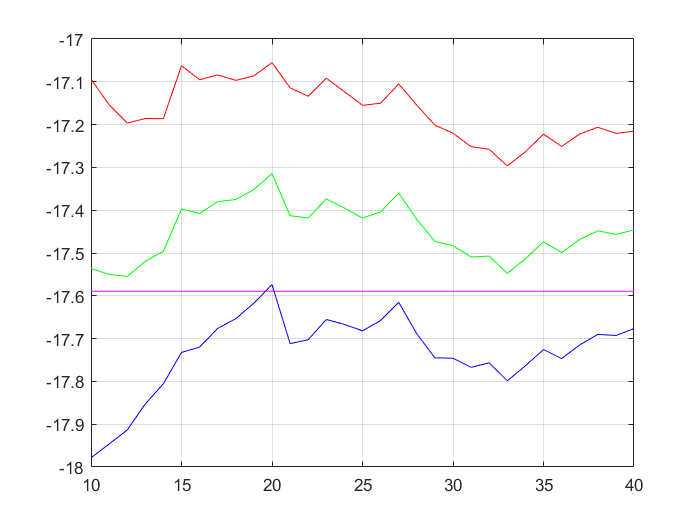
\includegraphics[scale=0.5]{untitled11}
\caption{График для задания 3a}
\label{fig:image}
\end{figure}

\begin{figure}[h!]
	\center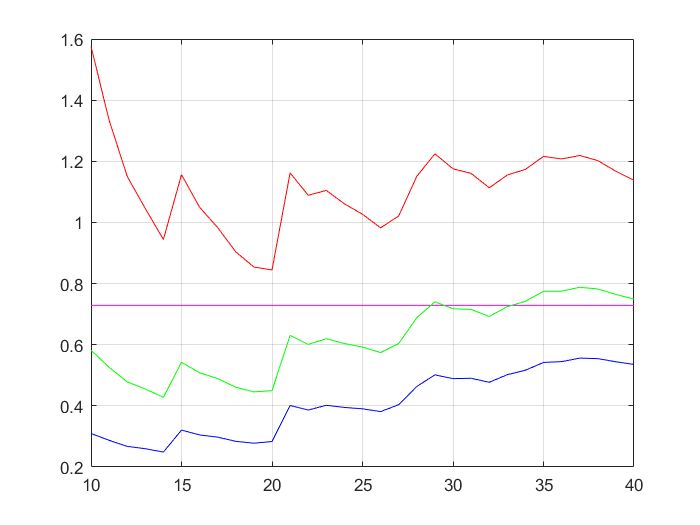
\includegraphics[scale=0.5]{untitled22}
	\caption{График для задания 3б}
	\label{fig:image1}
\end{figure}